% !TEX root = ./chemistry.tex

\chapter{Module 5 \; Equilibrium and Acid Reactions}

\section{Practical Investigation 2.1} \label{23/10/2024}
	Aim: To determine whether chemical reactions are reversible or not

	\subsection{Materials}
		\begin{itemize}
			\item 25 mL dropper bottle of \qty{1}{\moLar} cobalt(II) chloride hexahydrate
			\item 25 mL dropper bottle of \qty{0.05}{\moLar} potassium chromate
			\item 25 mL dropper bottle of \qty{0.05}{\moLar} potassium dichromate
			\item 25 mL dropper bottle of \qty{0.1}{\moLar} hydrochloric acid
			\item 25 mL dropper bottle of \qty{0.1}{\moLar} sodium hydroxide
			\item 1 $\times$ 5 cm piece of magnesium ribbon
			\item Distilled water
			\item 1 piece of filter paper (55 mm $\times$ 55 mm)
			\item 3 watch glasses
			\item 1 drying oven/incubator
			\item 4 test tubes
			\item Test-tube rack
			\item 4 small labels
			\item 1 pair brass tongs
			\item 1 $\times$ (5 cm $\times$ 5 cm) piece of sandpaper
			\item 1 $\times$ (5 cm $\times$ 5 cm) piece of steel wool
			\item Gas lighter
			\item Dropper
			\item Video camera
			\item Safety glasses and gloves
		\end{itemize}

	\subsection{Risk Assessment}
		\begin{table}[H]
			\centering
			\begin{tabular}{ll}
				\hline
				Hazard & Precaution \\ \hline
				Shattering glassware & Keep beakers, test tubes, and watch glasses in centre of table \\
				Exposure to harmful chemicals & Wear gloves and eye glasses. Handle with caution \\
				Burns from Bunsen burner & Keep on safety flame when not in use
			\end{tabular}
		\end{table}

	\subsection{Method}
		\subsubsection{Part A}
			\begin{enumerate}
				\item Place a piece of filter paper on a watch glass.
				\item Add cobalt chloride drop by drop until the filter paper is covered.
				\item Observe the colour of the filter paper.
				\item Place the watch glass into a drying oven overnight at \qty{35}{\degreeCelsius}.
				\item Remove the watch glass and filter paper and observe the colour of the filter paper.
				\item Add distilled water drop by drop to the same filter paper until it is covered.
				\item Observe the colour of the filter paper.
				\item Repeat steps 4 and 5.
			\end{enumerate}
		
		\subsubsection{Part B}
			\begin{enumerate}
				\item Label four test tubes A, B, C and D.
				\item Add about 1 mL of potassium chromate to test tubes A and B.
				\item Add about 1 mL of potassium dichromate to test tubes C and D.
				\item Test tubes A and C are reference solutions.
				\item Add hydrochloric acid dropwise to test tube B until a colour change occurs.
				\item Record your observations.
				\item Add sodium hydroxide dropwise to test tube B until another colour change occurs.
				\item Record observations.
				\item Add sodium hydroxide dropwise to test tube D until a colour change occurs. 
				\item Record observations.
				\item Add hydrochloric acid dropwise to test tube D until another colour change occurs.
				\item Record observations
			\end{enumerate}

			\subsubsection{Part C}
				\begin{enumerate}
					\item Clean a 5 cm piece of magnesium with sandpaper.
					\item Hold the piece of magnesium ribbon with a pair of brass tongs.
					\item Light the magnesium ribbon and hold it over a watch glass. Do not look directly at the magnesium while it is alight.
					\item Record observations.
				\end{enumerate}

			\subsubsection{Part D}
				\begin{enumerate}
					\item Hold a piece of steel wool with a pair of brass tongs.
					\item Light the steel wool and hold it over a watch glass.
					\item Record observations
				\end{enumerate}

			\subsection{Results}
				\subsubsection{Part A}
					\begin{itemize}
						\item When dehydrated, filter paper was blue when saturated with cobalt chloride
						\item When rehydrated, became pink
					\end{itemize}
					\begin{figure}[H]
						\centering
						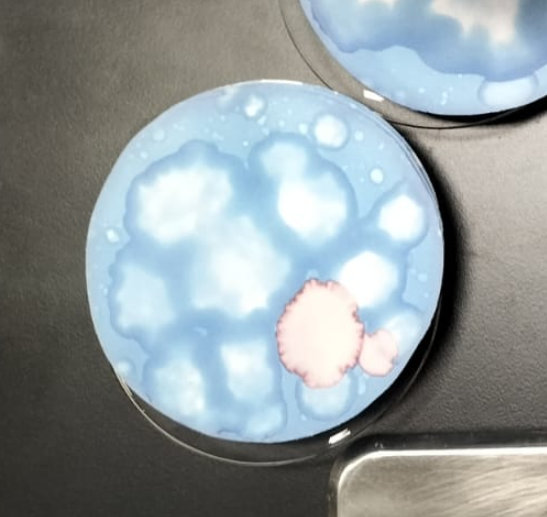
\includegraphics[width=7cm]{practical 2.1 part a.png}
					\end{figure}

				\subsubsection{Part B}
					\begin{itemize}
						\item Potassium chromate $\rightarrow$ initially bright yellow
						\item Potassium dichromate $\rightarrow$ initially orange
						\begin{itemize}
							\item $\ce{HCL} \rightarrow$ greenish-yellow
							\item $\ce{NaOH} \rightarrow$ darker yellow/orange
						\end{itemize}
						\item $\ce{2CrO4^{2-} + 2H+ <=> Cr2O72^{2-} + H2O}$
						\item $\ce{K2Cr2O7 + 2KOH <=> 2K2CrO4 + H2O}$
					\end{itemize}
				\subsubsection{Part C}
				\subsubsection{Part D}

\section{Le Chatelier's Principle} \label{29/10/2024-31/10/2024}
	"If a system at equilibrium is subject to a change in conditions, then the system will behave in such a way so as to partially counteract the imposed change"

	Haber process:

	\subsection{Effect of Concentration}
		\begin{equation}
			\ce{N2\gas{} + 3H2\gas{} <=> 2NH3\gas{} \quad \enthalpy{-92.5}}
		\end{equation}
		

	\subsection{Effect of Pressure}
	\subsection{Effect of Partial Pressure}
	\subsection{Effect of Volume}
		Decreasing the volume will increase the pressure. (Boyle's Law) This increases the collision rate between the reactants and favours the forward reaction.

	\subsection{Effect of Temperature}
		filler text
	
	\subsection{Summary}
		To use Le Chatelier's principle to predict the outcome of a change in conditions, you need to consider the following points.
		\begin{enumerate}
			\item What change is imposed?
			\item What is the opposite of the change?
			\item Which reaction direction is favoured - the forward or reverse?
			\item Does equilibrium shift to the left or right?
			\item What happens to the concentrations of each aqueous substance or gas?
		\end{enumerate}

	\begin{figure}[H]
		\centering
		\includegraphics{Le Chatelier's example problem}
	\end{figure}

	\textbf{D} When temperature decreases, the rates of both forward and backward reactions will decrease regardless of which way the endothermic or exothermic reaction goes. (A and B can be eliminated)

	This is because all the particles in the system lose kinetic energy, decreasing the rate of collisions hence, decreasing the rate of reaction.
	
	However, since there is a decrease in temperature the exothermic reaction will be favoured in order to counteract the change. In this case, the forward reaction being exothermic is affected less by the drop in temperature as shown in D.

\pagebreak
\section{Practical Investigation 2.3 - Effect of changes to concentration on equilibrium} \label{31/10/2024}

	Aim: To observe the effect of a change in concentration on a system at equilibrium

	\subsection{Materials}
		\begin{itemize}
			\item 2 mL of 0.1 molL$^{-1}$ iron(III) chloride solution
			\item 2 mL of 0.1 molL$^{-1}$ ammonium thiocyanate solution
			\item 1 mL of 0.1 molL$^{-1}$ calcium fluoride solution
			\item 20 mL distilled water
			\item 2x 10 mL measuring cylinders
			\item 25 mL measuring cylinder
			\item 4 test tubes
			\item Test-tube rack
			\item 4 small labels
			\item Disposable 1 mL droppers
			\item Waste bottle
			\item Digital camera
			\item Safety glasses
		\end{itemize}

	\subsection{Risk Assessment}
		\begin{table}[htbp]
			\centering
			\begin{tabular}{l|l}
				\hline
				Hazard & Precaution \\ \hline
				Chemicals may splash onto skin or eyes & Wear safety glasses and wash hands  \\
				Chemicals may harm aquatic life & Place in inorganic waste container \\
			\end{tabular}
		\end{table}

	\subsection{Method}
		\begin{enumerate}
			\item Pour 1 mL of iron(III) chloride solution into a 10 mL measuring cylinder.
			\item Pour 1 mL of ammonium thiocyanate into another 10 mL measuring cylinder.
			\item Pour both solutions into the 25 mL measuring cylinder.
			\item Add 18 mL of distilled water to the 25 mL measuring cylinder so that the total volume is 20 mL.
			\item Label four test tubes A, B, C and D.
			\item Pour equal volumes of the solution in the 25 mL measuring cylinder into each of the test tubes.
			\item Retain test tube A as the reference solution.
			\item Add 1 mL of iron(III) chloride to test tube B.
			\item Take a photo to record observations for test tube B relative to test tube A.
			\item Add 1 mL of ammonium thiocyanate to test tube C.
			\item Take a photo to record observations for test tube C relative to test tube A.
			\item Add 1 mL of calcium fluoride to test tube D. (Note: This reacts with the iron(III) ion so there is less iron(III) available to react with the thiocyanate ion.)
			\item Take a photo to record observations for test tube D relative to test tube A
		\end{enumerate}

	\subsection{Results}
		\begin{figure}[H]
			\centering
			\includegraphics{Practical Investigation 2.3 - Results.png}
			\caption{Test tubes A, B, C, D}
		\end{figure}

	\subsection{Discussion}
		\textbf{Explain each colour change in terms of collision theory.}

		The test tube B was darker in colour in comparison to test tube A. The increase in moles of reactants allows more successful collisions to occur, increasing the amount of product. The same principle applies to test tube C.

		Test tube D was lighter in colour compared to A, due to the calcium fluoride reacting with the iron (III) chloride 

	\subsection{Conclusion}
		\textbf{Use Le Chatelier's principle to explain what happened in test tubes B, C and D.}

		Test tube B was darker due to the increase in concentration of the reactant iron (III) chloride causes a shift of the equilibrium towards the products due Le Chatelier's principle
		
		Test tube C was darker due to the increase in concentration of the reactant ammonium thiocyanate causes a shift of the equilibrium towards the products due Le Chatelier's principle

		Test tube D was lighter because the calcium fluoride reacted with the iron (III) chloride, lowering the overall concentration of iron (III) chloride. This reduced the amount of reactants available, making the reverse reaction more favourable by Le Chatelier's principle.

\section{Calculating the Equilibrium Constant} \label{5/11/2024}
	The equilibrium constant can be used to predict the direction of chemical reactions

	$$K_{eq} = \frac{[products]}{[reactants]}$$
	For reaction:
	$$\ce{aA + bB <=> cC + dD}$$
	the equilibrium expression is:
	$$K_{eq}=\frac{[C]^{c}[D]^{d}}{[A]^a[B]^b}$$

	The concentration of each chemical species is raised to the power of the number of moles of that species indicated in the chemical equation. (Eg. there are $d$ moles of species $D$, hence in the equilibrium expression the concentration of species $D$ is raised to the power of $d$, written as $[D]^d$)

	\begin{itemize}
		\item The value for the equilibrium constant only takes into account the concentration of substances where the concentration can vary
		\item Solutions and gases can vary in concentration or partial pressure hence are included in $K_{eq}$
		\item Solids and pure liquids are NOT included eg. $\ce{H_2O}$ isn't required when calculating
	\end{itemize}

	\subsection{Reaction Quotient ($Q$)}
		$$Q=\frac{[C]^{c}[D]^{d}}{[A]^a[B]^b}$$
		Has the same formula as $K_{eq}$, however applies to any stage of a reaction
		
	\subsection{Equilibrium Constant}
		\begin{itemize}
			\item Comparing $Q$ to $K_{eq}$ predicts which way the equilibrium will shift
			\item $K_{eq}$ is where the equilibrium lies
			\item A large $K_{eq}$ means that there are more products than reactants; ie. equilibrium lies towards completion
			\item If $K_{eq}$ is close to one, both reactants and products are plentiful at equilibrium
		\end{itemize}
		\textbf{Example} Let $Q=2.1$, $K_{eq}=0.315$, $\therefore$ products$>$reactants.

	\subsection{Calculating the equilibrium expression}
		Consider the reaction between hydrogen and iodine producing hydrogen iodide:
		$$\ce{H_{2}\gas{} + I_{2}\gas{} <=> 2HI\gas}$$

\section{ICE Tables} \label{6/11/2024}
	\begin{table}[htbp]
		\centering
		\begin{tabular}{|l|l|l|l|}
			\hline
			 & [A] & [B] & [C] \\ \hline
			Initial concentration &  &  &  \\
			Change in concentration &  &  &  \\
			Equilibrium concentration &  &  &  \\ \hline
		\end{tabular}
	\end{table}

	$$\Delta c = c_{eq}- c_{u}$$

	Eg. $\ce{A + B <=> C + D}$

	\begin{table}[htbp]
		\centering
		\begin{tabular}{lllll}
			\hline
			 & [A] & [B] & [C] & [D]  \\ \hline
			Initial concentration 		& 0.6 & 0.6 & 0 & 0 \\
			Change in concentration 	& -0.5 & -0.5 & +0.5 & +0.5 \\
			Equilibrium concentration 	& 0.1 & 0.1 & 0.5 & 0.5 \\ \hline
		\end{tabular}
	\end{table}

	Eg. $\ce{2X \gas{} <=> 3Y \gas{} + 4Z \gas{}}$

	A sample consisting of 0.500 mol of X is placed into a system with a volume of 0.750 litres. \\
	At equilibrium, the amount of sample X is known to be 0.350 mol.

	\begin{table}[htbp]
		\centering
		\begin{tabular}{cccc}
			\hline
			 & X & Y & Z \\ \hline
			I 		& 0.5 & 0 & 0 \\
			C 		&  &  & \\
			E 		& 0.35 &  &  \\ \hline
		\end{tabular}
	\end{table}

	\begin{table}[htbp]
		\centering
		\begin{tabular}{cccc}
			\hline
			 	& X & Y & Z \\ \hline
			I 		& 0.5 & 0 & 0 \\
			C 		& -0.15 & -0.225 & +0.3 \\
			E 		& 0.35 & 0.225 & 0.3 \\ \hline
		\end{tabular}
	\end{table}

	\begin{align*}
		[X] &= \frac{0.35}{0.75} = 0.467 \\
		[Y] &= \frac{0.225}{0.75} = 0.3 \\
		[Z] &= \frac{0.3}{0.75} = 0.4
	\end{align*}
	
\section{Effect of Temperature on the Equilibrium Constant} \label{8/11/2024}
	Although other factors may affect equilibrium, $K_{eq}$ is only affected by temperature.
	Changing concentration, pressure, or volume will change the concentrations and therefore adjust the reaction point, however the reaction will still equalise to achieve the same $K_{eq}$

	\begin{itemize}
		\item For a particular reaction, $K_{eq}$ is constant at a given temperature
		\item Temperature changes the ratio of products and reactants, hence changing $K_{eq}$
		\item For $\ce{N2O2 \gas{} <=> 2NO2 \gas{}}$, temperature increases the $K_{eq}$ value and favours the formation of products. The forward reaction is endothermic
	\end{itemize}

	\subsection{Example Question}
		Nitric oxide gas ($\ce{NO}$) can be produced from the direct combination of nitrogen gas and oxygen gas in a reversible reaction.
		\begin{enumerate}
			\item \textbf{Write a balanced chemical equation for this reaction (1 mark)}
				\subitem $\ce{N2 \gas{} + O2 \gas{} <=> 2NO \gas{}}$
			\item \textbf{Explain, using collision theory, how an increase in temperature would affect the value for $K_{eq}$ for this system. Refer to the diagram in your answer.}
				\subitem An increase in temperature would favour the forward reaction, hence $K_{eq}$ will increase. More energy allows more collisions to occur
		\end{enumerate}
	
		\begin{align*}
			K_{eq} &= \frac{[p_1][p_2]}{[r_1][r_2]} \\
			1 &= \frac{[1][1]}{[1][1]} \\
		\end{align*}
		\text{\centering If $p_2$ decreases to $[0.5]$, favouring the forward reaction}
		\begin{align*}
			&= \frac{[1.15][0.65]}{[0.85][0.85]} \\
			&=K_{eq}
		\end{align*}

\section{Applications of the Equilibrium Constant} \label{12/11/2024}
	\subsection{Use of the Equilibrium Constant for the Dissociation of Ionic Solutions}
		Different ionic compounds have different solubilities

		Example reaction

		$$\ce{AgNO3 \aq{} + NaCl \aq{} -> AgCl \sld{} + NaNO3 \aq}$$

		Complete ionic equation: $\ce{Ag+ + NO3- +Na+ + Cl- -> AgCl \sld{} + NO3- + Na+}$

		Net ionic equation: $\ce{Ag+ \aq{} + Cl- \aq{} -> AgCl \sld{}}$

		Although a precipitate is formed, the reaction rests at a dynamic equilibrium where the rate at which the precipitate is formed is equal to the rate at which the ions are formed.

		$$\ce{AgCl \sld{} <=> Ag+ \aq{} Cl- \aq{}}$$

		\begin{itemize}
			\item By general practice, the solid precipitate is written on the left and the ions on the right.
			\item $K_{sp} = [\ce{Ag+}][\ce{Cl-}]$
			\item Since the solid is not included in the equilibrium constant, it is referred to as the \textbf{solubility product} ($K_{sp}$)
			\item If the system is not at equilibrium, it is referred to as the \textbf{ionic product}
			\item If $\text{ionic product} = K_{sp}$, then the system is at equilibrium.
			\item If $\text{ionic product} < K_{sp}$, the forward reaction would be favoured and the solid would dissolve for the system to reach equilibrium.
			\item If $\text{ionic product} > K_{sp}$, the reverse reaction would be favoured and more precipitate would form for the system to reach equilibrium.
		\end{itemize}

	\subsection{Use of the Equilibrium Constant for the Dissociation of Acids and Bases}
		\subsubsection{Acids}
			Strong acids dissociate completely in solution. The reaction goes to completion and is not an equilibrium system

			\subitem Eg: $\ce{HCl \lqd{} -> H+ \aq{} + Cl- \aq{}}$

			Weak acids do not dissociate completely, instead forming an equilibrium system

			\subitem Eg: $\ce{CH3COOH \aq{} <=> H+ \aq{} + CH3COO- \aq{}}$

			The acid dissociation constant is expressed as $K_a = \frac{[\ce{CH3COO-}][\ce{H+}]}{[\ce{CH3COOH}]}$

		\subsubsection{Bases}
			Strong bases dissociate completely in solution.

			\subitem Eg. $\ce{NaOH \sld{} -> Na+ \aq{} + OH- \aq{}}$

			Weak bases do not dissociate completely, only some of the molecules react with water to form ions, they form an equilibrium system

			\subitem Eg. $\ce{NH3 \aq{} + H2O \lqd{} <=> NH4+ \aq{} + OH- \aq{}}$
			
			The base dissociation constant is expressed as $K_b = \frac{[\ce{NH4+}][\ce{OH-}]}{[\ce{NH3}]}$

			\begin{figure}[H]
				\centering
				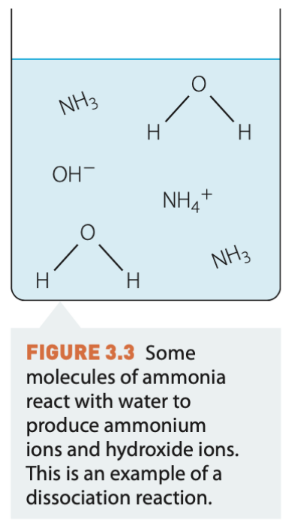
\includegraphics[width=5cm]{dissociation of bases.png}
			\end{figure}

		\begin{multicols}{2}
			\textbf{Weak Acid}

			General equation:
			$$\ce{HA \aq{} + H2O \lqd{} <=> H3O+ \aq{} + A- \aq{}}$$

			General expression for equilibrium constant:

			$$K_a = \frac{[\ce{H3O+}][\ce{A-}]}{\ce{HA}}$$
			
			\columnbreak

			\textbf{Weak Base}

			General equation:
			$$\ce{B \aq{} + H2O \lqd{} <=> BH+ \aq{} + OH- \aq{}}$$

			General expression for equilibrium constant:

			$$K_b = \frac{\ce{[BH+][OH-]}}{\ce{[B]}}$$
		\end{multicols}

	\subsection{Use of the Equilibrium Constant for Gaseous Systems}
		In a gaseous system (where all reactants are gases), the partial pressure of each species is related to its concentration ($c = \frac{n}{V}$)

		Pressure is due to the collisions between the gases and the walls of the container, therefore all particles within the system contribute to the pressure.

		The \textbf{partial pressure} is the proportion of the pressure due to collisions for a particular gas species

		For the general equation:

		$$\ce{aA \gas{} + bB \gas{} <=> cC \gas{} + dD \gas{}}$$, where $a$, $b$, $c$ and $d$ are the number of moles

		$$\text{Mole fraction of gas A} = \frac{\text{Number of moles of gas }}{\text{Total number of moles of gas present}}$$

		$$\text{Partial pressure of gas A} = \text{Mole fraction of gas A} \times \text{Total pressure of the system}$$

		Expression of equilibrium constant in terms of pressure:
		$$K_p = \frac{P^a_A \times P^b_B}{P^c_C \times P^d_D}$$

\section{Beer Lambert Law} \label{14/11/2024}
	\begin{align*}
		\text{Absorbance (for a given wavelength)} &= \text{Molar absorbility} \times \text{Path length} \times \text{Concentration} \\
		A &= \varepsilon lc
	\end{align*}
	\begin{itemize}
		\item Absorbance has a direct relationship to concentration
		\item Greater concentration, greater absorbance
	\end{itemize}

	Absorbance can be measured using a spectrophotometer (for all wavelengths) or a colourimeter (for the visible spectrum). Using the formula, the absorbance coefficient ($\varepsilon$) for a given material can be calculated. The coefficient determines how far light can penetrate a material before it is absorbed, depending on the material and the wavelength being absorbed. Measured in $\unit{\L\per\mole\per\cm}$

	A filter is applied to the light and must be the complement to the colour of the solution.

	Eg: For reaction $\ce{Fe3+ \aq{} + SCN- \aq{} <=> FeSCN2+ \aq{}}$
	$\ce{FeSCN}$ is red, $\therefore$ a green filter is needed

	\begin{figure}[H]
		\centering
		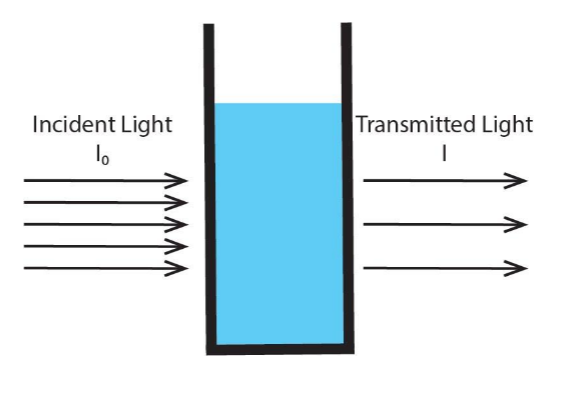
\includegraphics[width=10cm]{absorption coefficient.png}
	\end{figure}

	\begingroup
		\Large
		\begin{align*}
			A = \log_{10}{\frac{I_o}{I}} = \varepsilon lc
		\end{align*}
	\endgroup

	\newpage

	\subsection{Worked Example}
		A solution thickness of 1 cm transmits 30\% incident light.
		\begin{enumerate}
			\item \textbf{Calculate the concentration of the solution given the molar absorptivity of the solution being 4000 L mol$^{-1}$ cm$^{-1}$}
			
			\begin{align*}
				A = \log_{10}{\frac{100}{30}} = 0.523 \\
				\therefore C = \frac{A}{\varepsilon l} &= \frac{0.523}{4000 \times 1} \\
				&= \SI{1.31e-4}{\mole\per\litre}
			\end{align*}

			\item \textbf{Calculate the molar absorptivity of a $\SI{1e-4}{\mol\per\litre}$ solution which has an absorbance of 0.20, when the path length is 2.5 cm.}
			
			\begin{align*}
				A &= \varepsilon l c \\
				0.2 &= 1 \times 10^{-4} \times 2.5 \times \varepsilon \\
				\varepsilon &= \frac{0.2}{1 \times 10^{-4} \times 2.5} \\
				&= {800} \unit{\litre\per\mole\per\cm}
			\end{align*}

			\item \textbf{Which instrument is used in the verification of Lambert's Beer's law?}
			\subitem Colourimeter

			\item \textbf{Find out the molar absorptivity of a $\SI{1e-4}{\mole\per\litre}$ solution with an absorbance of 0.30, when the path length is 1.5 cm. (3 marks)}
			
			\begin{align*}
				A &= \varepsilon lc \\
				0.3 &= \varepsilon \times 1.5 \times 1 \times 10^{-4} \\
				\varepsilon &= 2000 \unit{\litre\per\mole\per\cm}
			\end{align*}
		\end{enumerate}

	\subsection{Colourimeters}
		In order to determine concentration of a solution from its absorbance, a calibration curve using known concentrations and absorbances must be used to interpolate or extrapolate datapoints corresponding to a desired value.

		\begin{figure}[H]
			\centering
			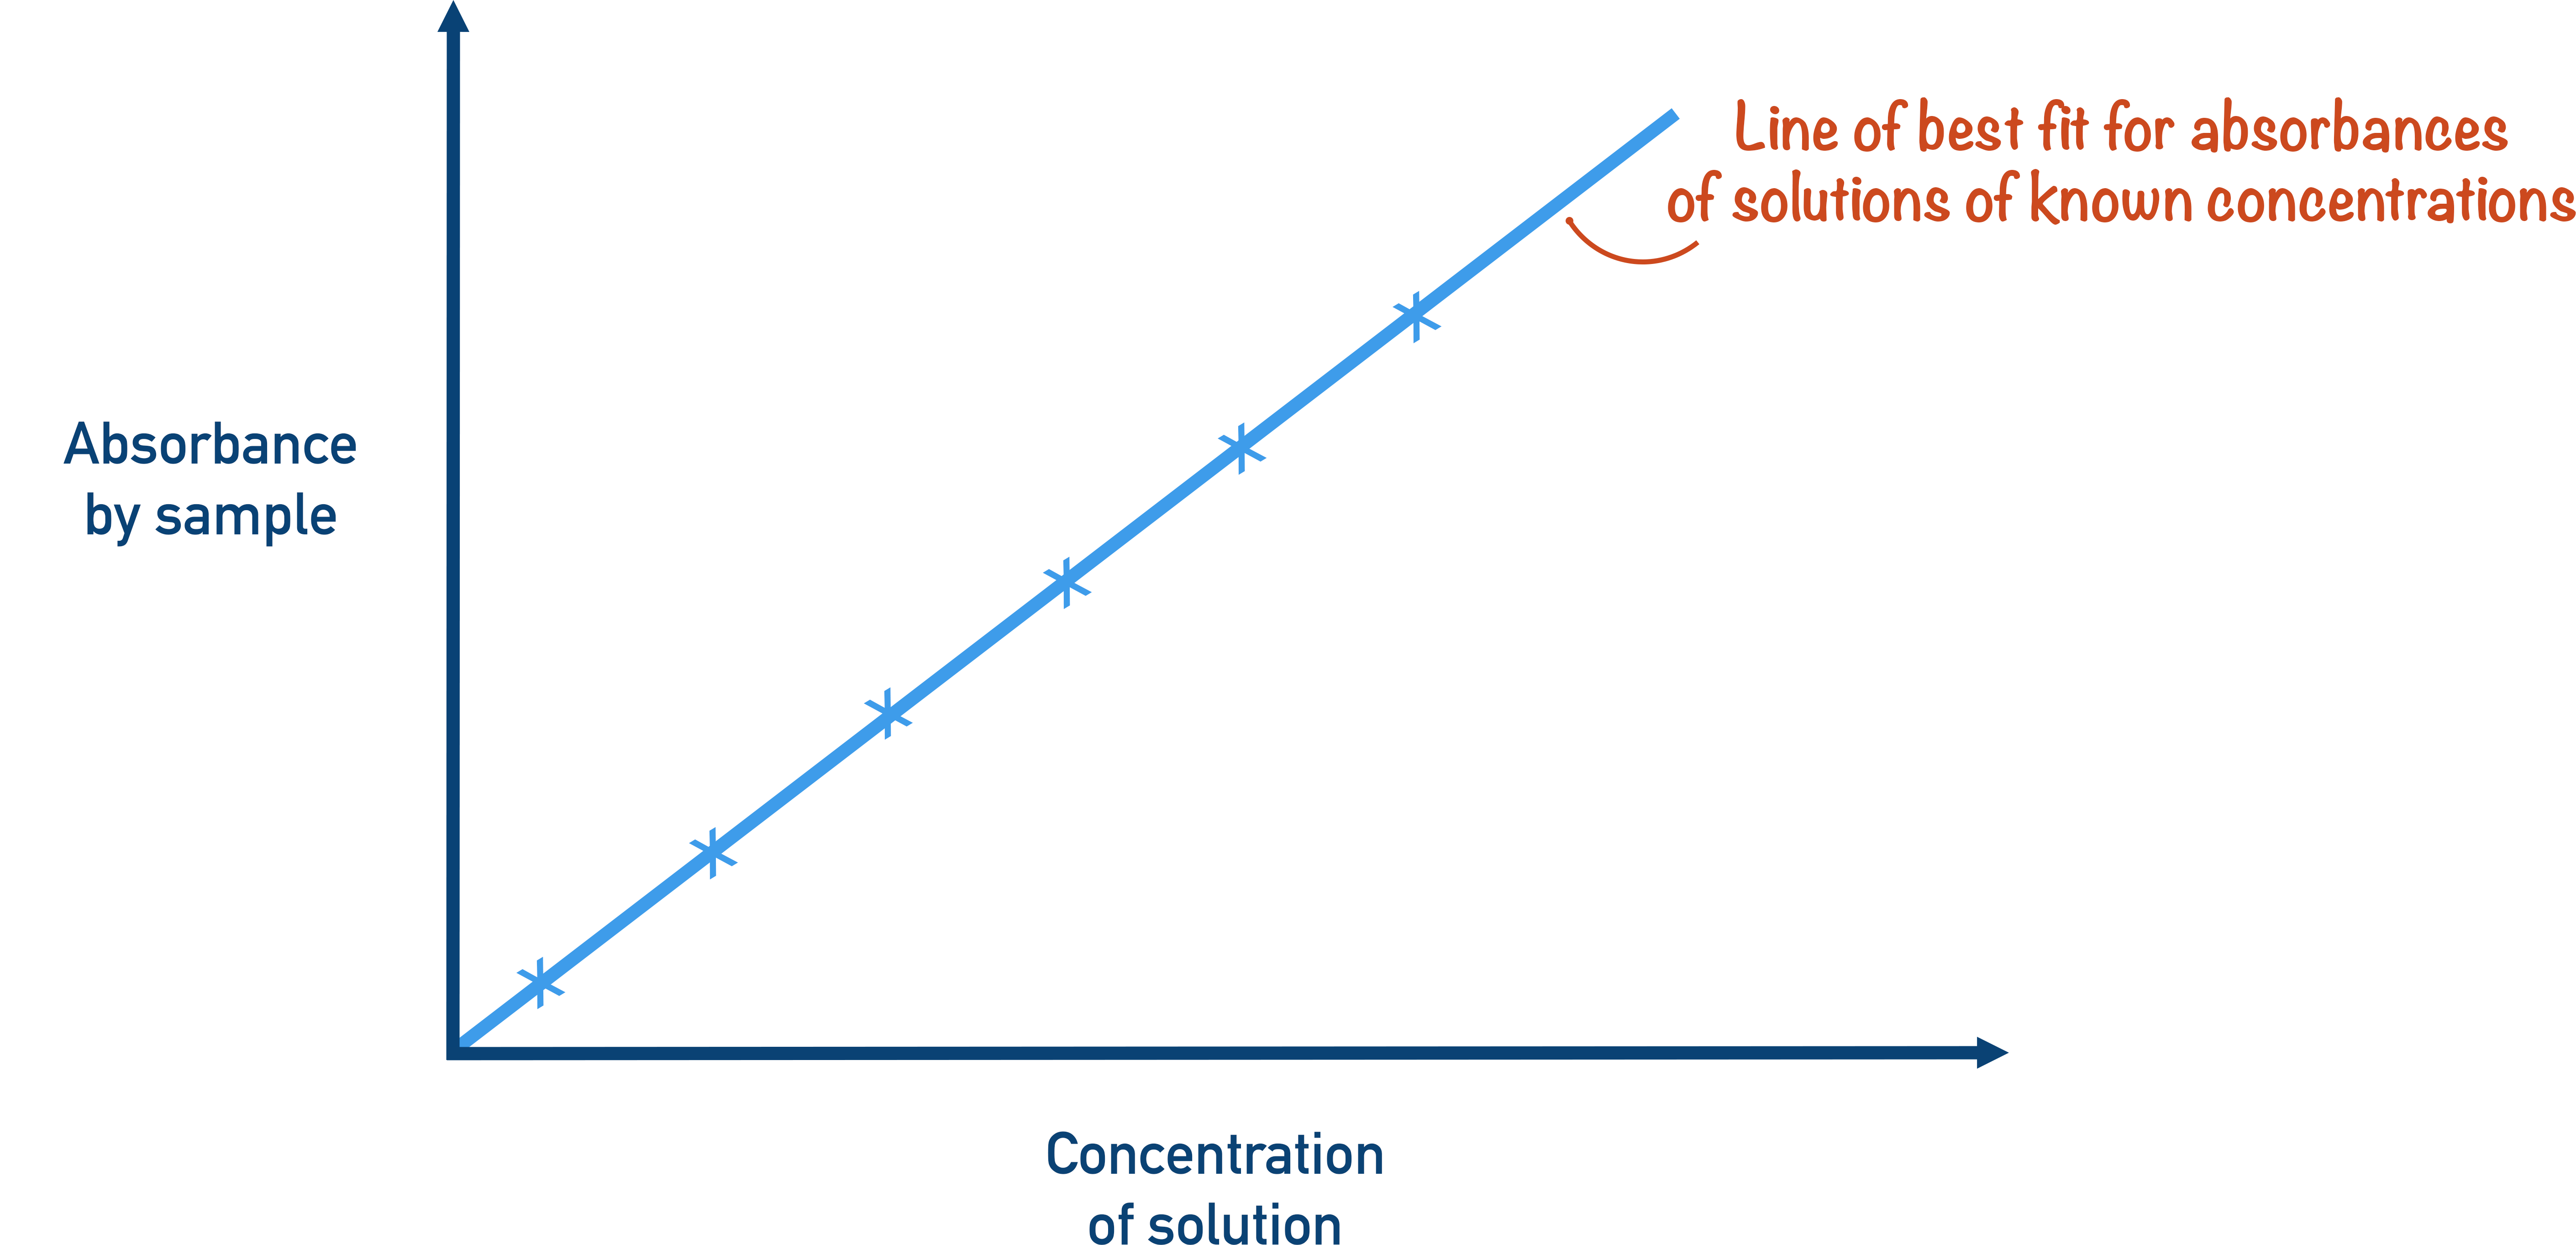
\includegraphics[height=7cm]{calibration curve.png}
		\end{figure}

		Beer Lambert's Law collapses at high and low concentrations, where $c<20\%$, $c>80\%$
	
	\section{Practical Investigation 3.2}
	Aim: To use colourimetry to determine the equilibrium constant for the reaction of iron(III) ions with thiocyanate ions to form the iron(III) thiocyanate ion

	\subsection{Materials}
		\begin{itemize}
			\item 200 mL 0.2 \unit{\moLar} $\ce{Fe(NO3)3}$
			\item 100 mL 0.002 \unit{\moLar} $\ce{KSCN}$
			\item 500 mL 0.5 \unit{\moLar} $\ce{HNO3}$
			\item 60 mL 0.002 \unit{\moLar} $\ce{Fe(NO3)3}$
			\item 150 mL distilled water
			\item 6 * 100 mL volumetric flasks
			\item 5 * 150 mL beakers
			\item 2 * 100 mL beakers
			\item 1 * 25 mL bulb pipette
			\item 2 * 10 mL graduated pipettes
			\item 1 * 10 mL bulb pipette
			\item 2 pipette bulbs
			\item 1 disposable pipette
			\item Waste bottle
			\item 14 small labels
			\item 1 colourimeter and set of cuvettes
			\item Safety glasses
		\end{itemize}

	\subsection{Risk Assessment}
		\begin{table}[htbp]
			\centering
			\begin{tabular}{ll}
				\hline
				Hazard & Precaution \\ \hline
				Breaking glassware & Keep glassware on inside of table, do not run with glassware \\
				Spillage of solutions & Handle with caution, clean any spills immediately \\
				Splashing of solution into eyes & Wear safety goggles \\ \hline
			\end{tabular}
		\end{table}
	
	\subsection{Method}
	\begin{enumerate}
		\item Label the six volumetric flasks A-F.
		\item Use a 25 mL bulb pipette to transfer 25.00 mL of the 0.200 \unit{\moLar} $\ce{Fe(NO3)}$\item 3 to flask A.
		\item Use a graduated 10 mL pipette to transfer 1.00 mL of the 0.002 \unit{\moLar} \item $\ce{KSCN}$ to flask A.
		\item Add HNO3 to make a final volume of 100.00 mL.
		\item Make solutions with known concentration by pushing equilibrium as far as possible to the products. $\ce{HNO3}$ can be used to reduce the concentration of $\ce{H3O}$
		\item Rinse the cuvette with distilled water.
		\item $\frac{3}{4}$ fill the cuvette with distilled water and wipe the clear sides. 
		\item Turn on the colourimeter and turn the light to blue or 470 nm.
		\item Use the cuvette with distilled water to calibrate the colourimeter. Note: Orientate the cuvette correctly in the colourimeter so that the light passes through the clear sides of the cuvette.
		\item Rinse, a 100 mL beaker with standard solution A - it is easier to pour the solution into the cuvette using a beaker than using a volumetric flask.
		\item Rinse, then $\frac{3}{4}$ fill the cuvette with standard solution A and measure the absorbance with the colourimeter.
		\item Repeat steps 10 and 11 for the other standard solutions (B-F)
	\end{enumerate}

\section{Solution Equilibria - Dissolution of Ionic Compounds} \label{19/11/2024}
	\subsection{Solubility Revision}
		\begin{itemize}
			\item Ionic compounds consist of a positive cation and negative anion
			\item Due to the polar nature of water molecules, they can arrange themselves around the ions and overcome the ionic bonding, dissolving the substance into an aqueous solution
			\item When surrounded by water, the ion becomes a \textbf{hydrated ion}
			\item For an ionic compound to dissolve, the energy required has to be less than or similar to the energy released when hydrated
		\end{itemize}

		$$\text{Energy to break lattice} \approx \text{Energy released when ions hydrated}$$

		Solubility can be measured in \unit{\gram\per\litre}, g/100 g, or g/100 mL

	\subsection{Factors influencing solubility}
		\begin{itemize}
			\item Activation energy required to break lattice
				\item Strength of ionic bonding
				\item Size of ions
				\item Charge of ions
		\end{itemize}

	\subsection{Solubility}
		\begin{itemize}
			\item The solubility of a solute is the maximum mass in grams that can dissolve in 100 g of the solvent at a given temperature (\unit{\gram\per\litre} can also be used)
			\item A solution is saturated when no more solute will dissolve at a given temperature
			\item Heat will increase the solubility of a solute
			\item Solubility curves show how much of a solute dissolves at a given temperature
		\end{itemize}
		\begin{figure}[H]
			\centering
			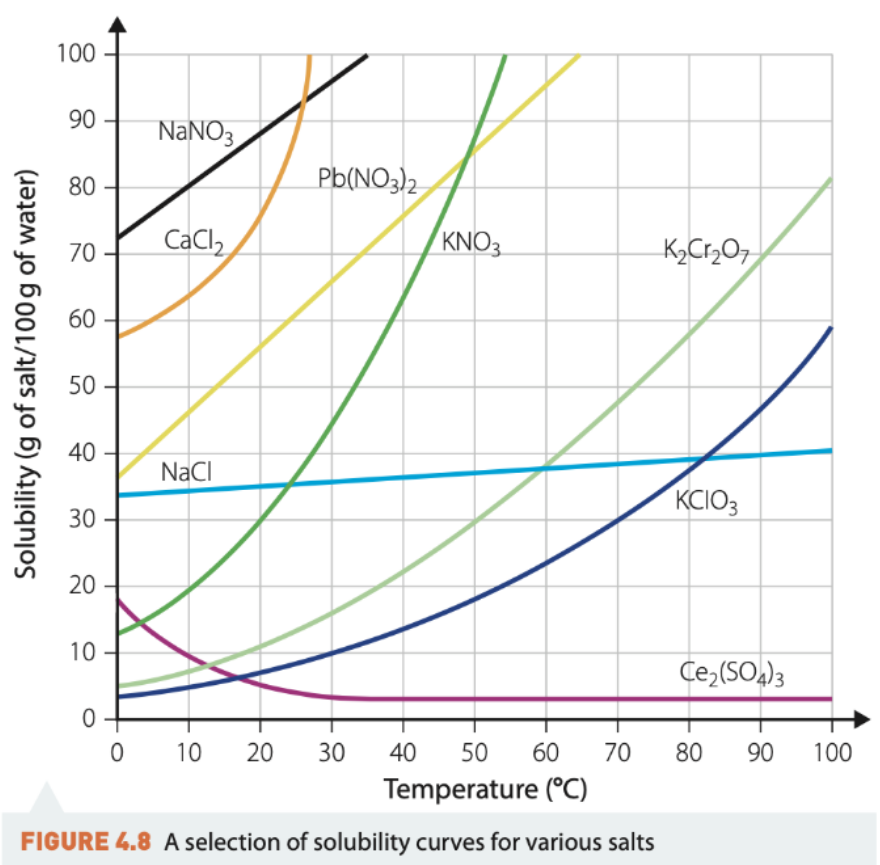
\includegraphics[width=10cm]{solubility curve.png}
		\end{figure}

	\subsection{Water of Crystallisation}
		Water of crystallisation occurs when water molecules are attracted to the ions of a salt

		Eg. $\ce{CuSO4 . 5H2O}$ is a substance with five water molecules of crystallisation per unit of copper (II) sulphate

		Water or other molecules that form dipole bonds to a metal atom are referred to as ligands

		The water of crystallisation can be evaporated by heating the hydrated compound and the product is said to be anhydrous

	\subsection{Toxins in Cycad Fruit}
		Cycad plants are native Australian trees that produce fruits that contain seeds with cone-like structures. There are several types, however most fruits and seeds are poisonous.

		They contain two main toxins; cycasin and beta-methylamino-L-alanine (BMAA)

		Cycasin and BMAA are types of azoxy glycosides, a group of toxins known to cause severe gastrointestinal issues in humans. These toxins can cause severe liver disorders and impact the functioning of nerves, leading to ataxia.

		Cycasin and BMMA are water-soluble and can be dissolved out of the seeds and into the surrounding water.

		\textbf{Leaching} involves placing the fruit in water and leaving it to soak, removing the toxins

		$$\ce{\text{Cycasin} \sld{} <=> \text{Cyasin} \aq{}}$$

		In the above equilibrium, the concentration of toxins in the water is initially zero. By Le Chatelier's Principle, the equilibrium shifts to the right, decreasing the high concentration of solid toxins in the fruit, eventually reaching a dynamic equilibrium. Although some toxins are removed, the system reaches an equilibrium where toxins are still present. To improve the result, running water can be used (ie. an open system) so that the system can never reach an equilibrium. The equilibrium will constantly shift to the right, hence removing most toxins from the seed and fruit.

		\text{\Large Other Methods}
		\textbf{Cooking} cycad fruit causes the toxins to decompose due to the intense heat.
		\textbf{Fermenting} cycad fruit sees natural processes break toxins down over time.

\section{Measuring Solubility} \label{20/11/2024}
	\begin{itemize}
		\item The mass of a substance that dissolves depends upon temperature.
		\item The solubility of a solute is the maximum mass in grams that can dissolve in 100 g of the solvent at a given temperature.
		\item Unsaturated solution
		\item Saturated - solid stays at bottom
		\item Supersaturated - more solute dissolved than in a saturated solution at the same temperature.
		\begin{itemize}
			\item If this supersaturated solution is bumped, sugar crystal is added or the side of the glass is scratched, then the extra sugar will precipitate out again.
		\end{itemize}
	\end{itemize}

	\begin{figure}[H]
		\centering
		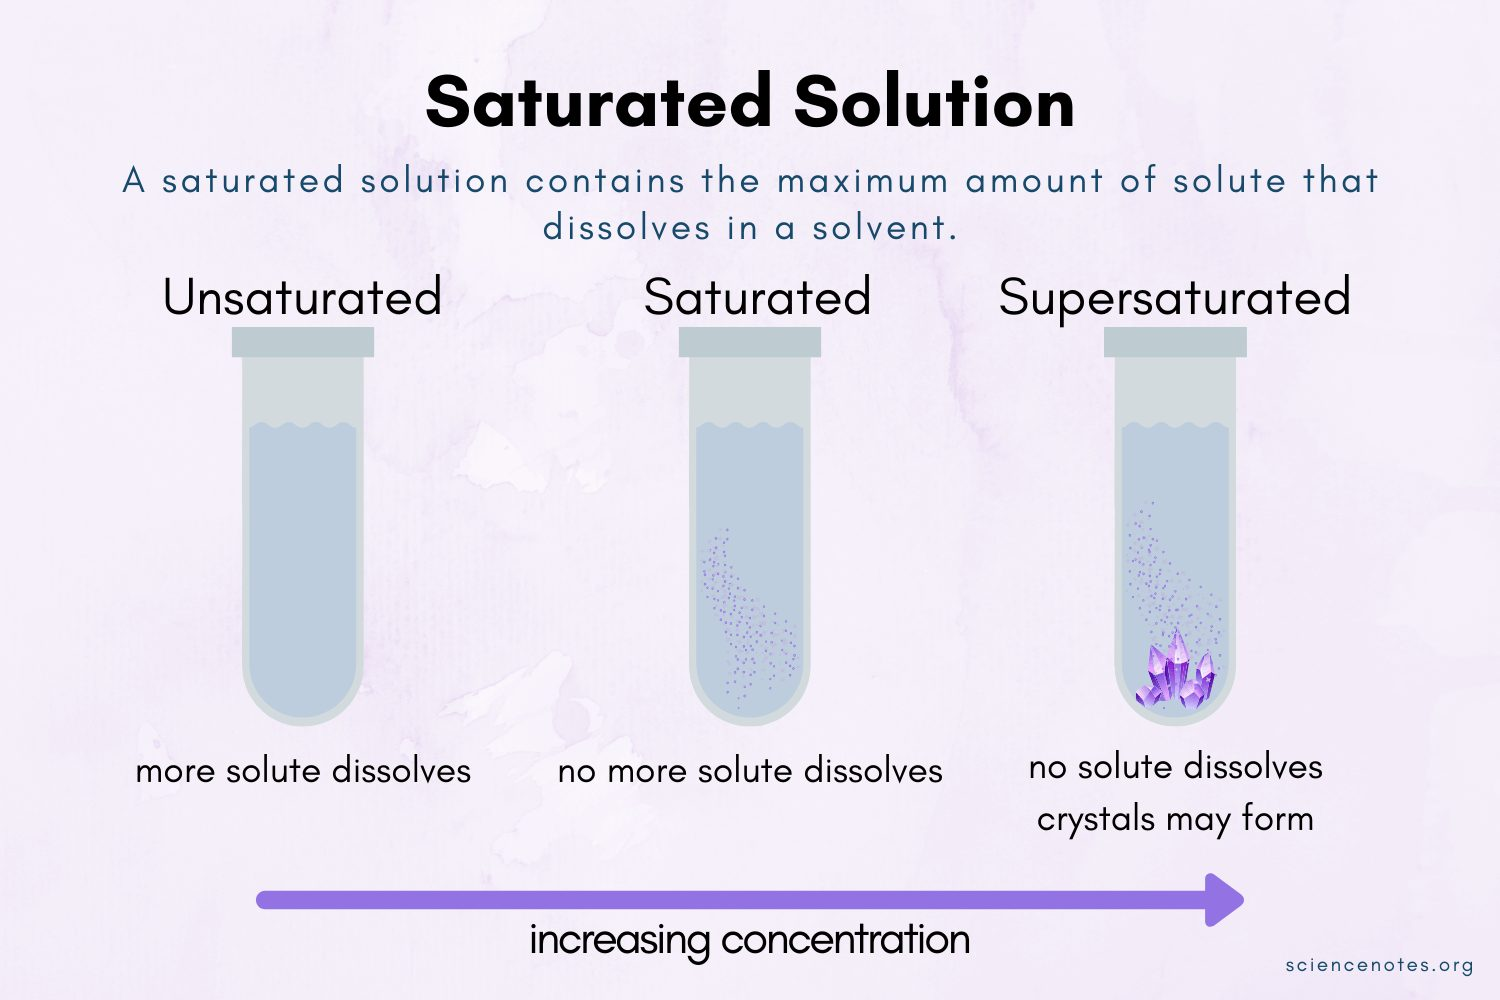
\includegraphics[width=14cm]{saturated solution.jpg}
	\end{figure}

	\subsection{Solubility Rules}
		\begin{itemize}
			\item Solutions of substances dissolved in water are called aqueous solutions. The term "aqueous" comes from the Latin aqua, meaning water.
			
			When ionic substances dissolve in water, they dissociate. This means they separate into their ions, which are then able to move freely and independently of each other through the solution.
			
			Although most ionic compounds are soluble in water, they do not all dissolve to the
			same extent.
			
			"Soluble" means that a compound dissolves to more than 10 g L-1 (or 1 g/100 mL),
			
			"insoluble" means that it dissolves to less than 1 g L-1, and
			
			"sparingly soluble" means that it dissolves in the range 1 g L-1 to 10 g L-1 .
		\end{itemize}
\section{Solubility Product}


\section{Practical Investigation 4.2 - Deriving the solubility curve for potassium chloride}
	Aim: To gather data to draw a solubility curve for potassium chloride

	\subsection{Materials}
		\begin{itemize}
			\item Potassium chloride
			\item Distilled water
			\item 250 mL
			\item 10 mL measuring cylinder
			\item Large test tubes
			\item Bunsen burner
			\item Tripod
			\item Gauze mat
			\item Bosshead and clamp
			\item Retort stand
			\item -10-110 $\unit{\degreeCelsius}$ thermometer
			\item Stirring rod
			\item Balance
			\item Weighing bottle
			\item Matches
			\item Test-tube rack
			\item Wire gauze
			\item Spatula
			\item Safety glasses
		\end{itemize}

	\subsection{Risk Assessment}
		\begin{table}[H]
			\centering
			\begin{tabular}{ll}
				\hline
				Hazard & Precaution \\ \hline
				Burning from Bunsen burner & Do not use the Bunsen burner if the gas tube is damaged. \\
				Poison from chemicals & Do not drink chemicals \\
				Spillage of chemicals & Keep beakers in centre of table. Handle with caution
			\end{tabular}
		\end{table}

	\subsection{Scientific Diagram}

		\begin{figure}[H]
			\centering
			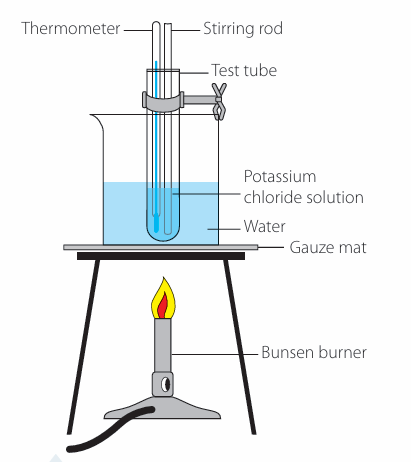
\includegraphics[width=14cm]{4.2 practical diagram.png}
			\caption{Use retort stand instead of beaker clip}
		\end{figure}
	
	\newpage
	
	\subsection{Results}
		\begin{table}[H]
		\centering
			\begin{tabular}{llll}
			\hline
			Mass of $\ce{KCl}$ (g) 		& $m_{water}$ (g)		& Temp. recrystallisation ($\unit{\degreeCelsius}$)	& Solubility (g/100 g $\ce{H2O}$)	\\ \hline
			3.00						& 10.00					& 57 												& 30								\\
			3.40						& 10.00					& 65 												& 34								\\
			3.80						& 10.00					& 69 												& 38								\\
			4.20						& 10.00					& 86 												& 42 								\\ \hline
			\end{tabular}
		\end{table}

	\subsection{Analysis of Results}
		\begin{enumerate}
			\item \textbf{Use the class results to plot a graph of solubility against temperature. Plot the temperature along the horizontal axis (0-100°C).}
			\begin{figure}[H]
				\centering
				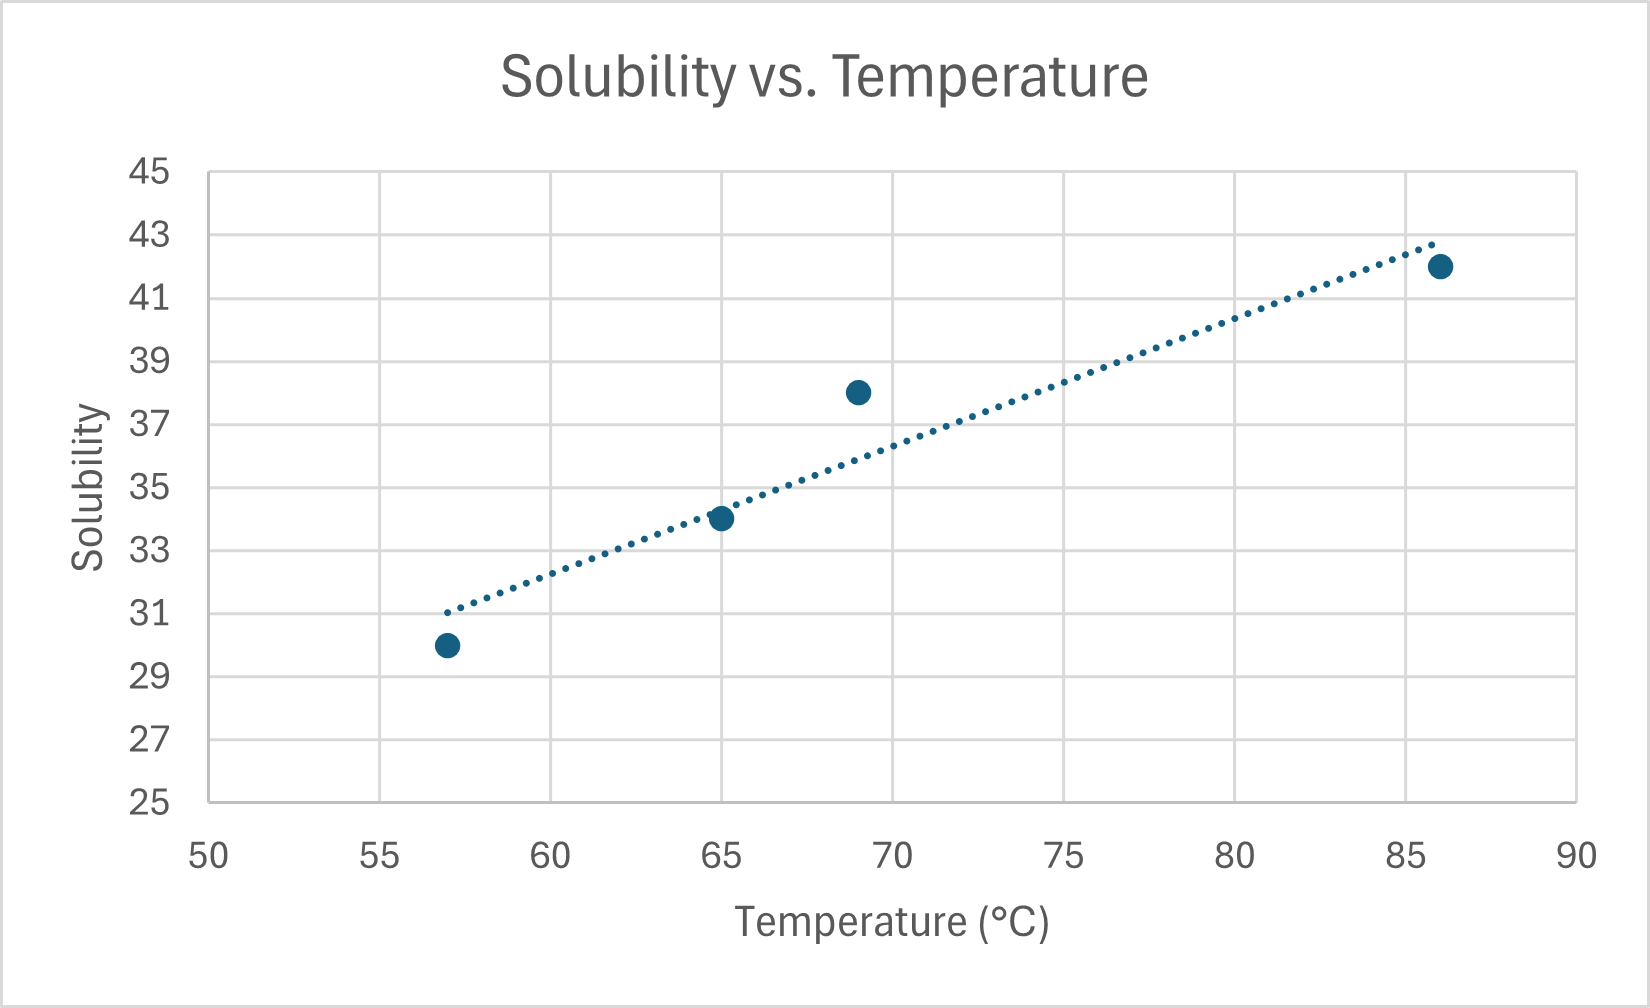
\includegraphics[width=14cm]{solubility temperature graph.png}
			\end{figure}
			\item \textbf{From the graph, predict the solubility of potassium chloride at 20 $\unit{\degreeCelsius}$ 40 $\unit{\degreeCelsius}$, 60 $\unit{\degreeCelsius}$ and 80 $\unit{\degreeCelsius}$.}
				\subitem By technology, trendline forms equation $\text{Solubility} = 0.4056T + 7.9142$

				\begin{align*}
					\text{Solubility at 20} \unit{\degreeCelsius} &= 0.4056(20) + 7.9142 \\
					&= 16.0262 \unit{\solub}
				\end{align*}
				\begin{align*}
					\text{Solubility at 40} \unit{\degreeCelsius} &= 0.4056(40) + 7.9142 \\
					&= 24.1382
				\end{align*}
				\begin{align*}
					\text{Solubility at 60} \unit{\degreeCelsius} &= 0.4056(60) + 7.9142 \\
					&= 32.2502
				\end{align*}
				\begin{align*}
					\text{Solubility at 80} \unit{\degreeCelsius} &= 0.4056(80) + 7.9142 \\
					&= 40.3622
				\end{align*}
		\end{enumerate}

	\newpage

	\subsection{Discussion}
		\begin{enumerate}
			\item \textbf{Describe what happens to the solubility of potassium chloride as temperature increases}
				\subitem As temperature increases, solubility of potassium chloride increases, ie. directly proportional relationship
			\item \textbf{If the theoretical value for the solubility of potassium chloride at \qty{50}{\degreeCelsius} is \qty{50}{\solub}, what percentage error does your experiment have?}
			$$\text{Percentage error} = \frac{\text{Experimental value} - \text{true value}}{\text{True value}} \times 100\%$$

			\begin{align*}
				\text{Solubility at 50} \unit{\degreeCelsius} &= 0.4056(50) + 7.9142 \\
				&= 28.1942
			\end{align*}

			\begin{align*}
				\text{Percentage error} &= \frac{28.1842 - 50}{50} \times 100 \\
				&= \frac{-21.8158}{50} \times 100 \\
				&= -43.6316 \% \\
				&\therefore \text{The experiment had a error value of 43.6316 \%}
			\end{align*}
			
			\item \textbf{List possible sources of errors in your experiment.}
				\begin{itemize}
					\item Observing the formation of precipitate was subjective as small particles initially formed
					\item The water bath helped to regulate the temperature of the test tube, however may not have been fully effective
				\end{itemize}
		\end{enumerate}